\section*{Implementation}
% Explain general layout:
% Packet header structure and message types (make a graph)
% two phases: sleep and active 
% messages are set in a readyQueue and sendQueue which user of library can access
% functions are all nonblocking except QMAC.run(), where all messages are sent

% Explain how active phase scheduling works (make a graph):
% explain why have chosen random slot allocation -> no leader needed compared to other TDMA protocols.  mention that we have also tried CSMA but we encountered a kind of deadlock

% Explain how synchronization mode works:
% Explain why we chose the intervallength and when to call synchronize(). Explain what problems would arise if we did it in another way.

This project was tested on two Lilygo TTGO T-BEAM V1.1 boards, equipped with LoRa and GPS modules and capable of battery power. In this project, only the LoRa module was used. A library implementing the QMAC protocol was developed in C++ using the Platformio framework. The following sections will explain the workings of the QMAC protocol in detail.


\subsection*{Packet Structure}

The QMAC packet structure is illustrated in Figure 1. Each packet header consists of four bytes, with one byte per field. The payload ranges from 1 to 211 bytes, and a CRC checksum of two bytes is appended for error detection. Special packets include ACK and SYNC packets. An ACK packet has a payload length of 0, resulting in a total size of 6 bytes. A SYNC packet, identified by a packet ID of 0, includes a duration field with 2 bytes instead of the payload length, making its total size 7 bytes. The limited one-byte fields for destination, source, and packet ID restrict the addressing to 255 devices and 254 unique message IDs. This would have to be adjusted for larger networks.


\begin{figure}[h]
	\centering
	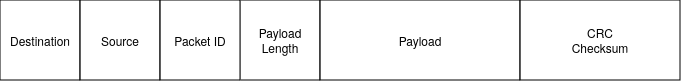
\includegraphics[width=\textwidth]{figures/packet.png}
	\caption{Structure of a QMAC packet}
\end{figure}

\subsection*{Overview of States}
A device can be in three states: Sleeping, active or synchronizing.
\begin{itemize}
	\item \textbf{Sleeping State} In the sleeping state, the LoRa module is powered off. During this phase, the device can execute code unrelated to the protocol.
	      Users of the library can enqueue packets for future transmission and query packets that have been received.
	\item \textbf{Active State} After a predefined interval, known as \textit{sleepDuration}, a timer interrupt will trigger, transitioning the device into the active state for another predefined interval, referred to as \textit{activeDuration}. The user must periodically invoke the function \texttt{QMAC.run()}.
	      This function is essential for executing the protocol's operations during the active phase.
	      If the device is not in the active state, the function simply returns without performing any actions. Upon entering the \texttt{run()} function, packet transmission is scheduled. Subsequently, packets are sent according to this schedule, and the device listens and responds based on the types of packets received. After another timer interrupt, the device normally goes back into the Sleeping state.
	\item \textbf{Synchronizing State} The synchronizing state aims to achieve consensus among nodes regarding the start of the active phase. The device enters this state under any of the following conditions: during the initialization of the QMAC library, if the ratio of unacknowledged packets exceeds a specified threshold, or after a predetermined number of cycles (defined as \textit{sleepDuration} + \textit{activeDuration}). In this state, the module transmits SYNC packets for at least one cycle and continues until a SYNC response is received. Based on the SYNC responses, the device estimates when other nodes will transition to the active state and then returns to the Sleeping state until the estimated time.
\end{itemize}


\begin{figure}[h]
	\centering
	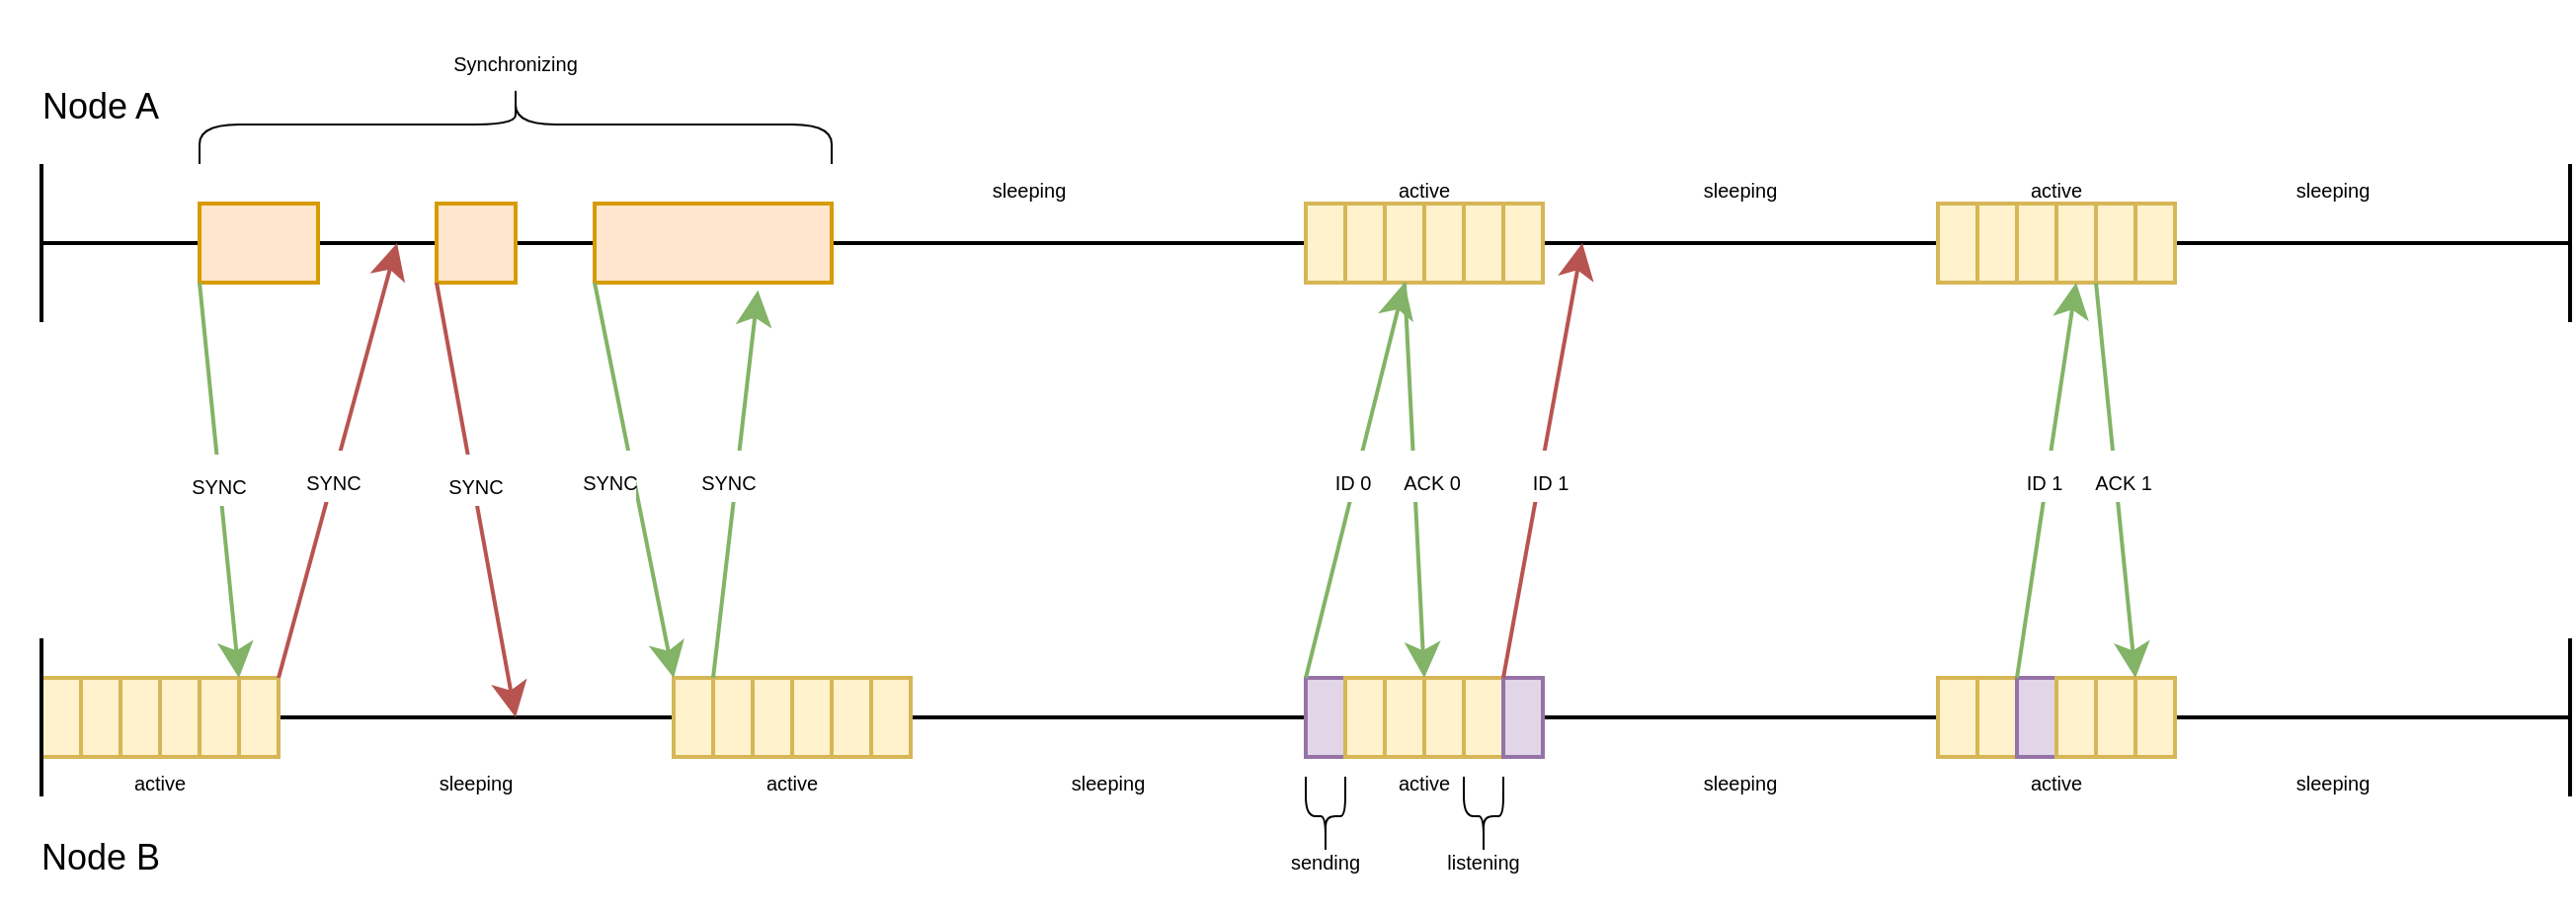
\includegraphics[width=\textwidth]{figures/qmac-time.png}
	\caption{Device States}
\end{figure}

\subsection*{The Active Phase}

In the active phase, similar to the TSMP protocol, the duration is divided into fixed-sized time slots. Within each slot, a node is either receiving or sending. At the start of the active phase, the transmission of packets queued by the library user is scheduled. Unlike other MAC protocols, QMAC does not have a leader to dictate the timing of message transmissions. Instead, each slot is numbered, and packets are assigned specific slot numbers. Packets are sent in their designated slots. The disadvantage of this approach is that this can lead to collisions if multiple nodes select the same slot for sending. However, this method eliminates the need for a leader or an agreement process among the nodes.

After transmitting a packet, it is placed in a resend queue, awaiting an ACK packet with the same packet ID. If the ACK is received, the packet is removed from the resend queue. At the end of the active phase, packets remaining in the resend queue are transferred to the send queue for retransmission in future active phases. Users can configure the retransmission policy to drop unacknowledged packets after a specified number of cycles, preventing indefinite queue growth.

During listening slots, the device processes incoming packets based on their type. ACK packets lead to the removal of corresponding packets from the resend queue. SYNC packets trigger a SYNC response, indicating the duration in milliseconds until the next active phase begins. Payload packets are added to the reception queue for user retrieval during the sleep phase.


\subsection*{The Synchronization Phase}

During the synchronization phase, a node transmits SYNC packets for at least one full cycle duration or until a SYNC packet is received. The interval at which it sends SYNC packets is randomized but less than the active duration. This ensures that the node will eventually send a packet when a neighboring node is active and capable of responding with a SYNC packet. \\

The node transmits SYNC packets for at least one full cycle duration to ensure it receives responses from all nodes, which may have very different active phases. If the node stopped transmission after receiving the first SYNC packet, it could result in clusters of synchronized nodes that are not synchronized with each other.

\begin{figure}[h]
	\centering
	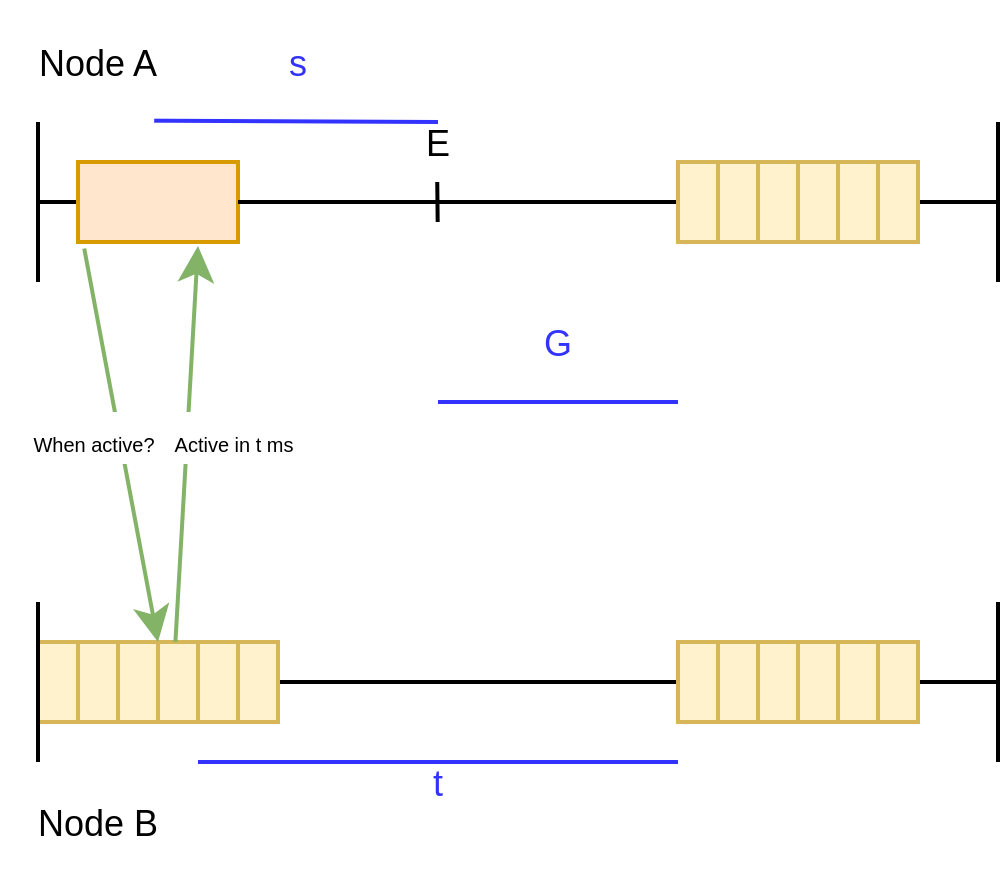
\includegraphics[width=0.5\textwidth]{figures/synchronization.png}
	\caption{Visualization of calculation parameters}
\end{figure}

After the cycle duration, and upon receiving packets, the node evaluates the timing of the next active phase based on the received durations, using a method similar to the GTSP protocol. The node performs the following calculations: Let \( E \) represent the time of evaluaton, \( r_1, \ldots, r_n \) denote the times when the querying node received SYNC packets, and \( d_1, \ldots, d_n \) signify the response times (the durations it took to receive the SYNC responses). For each response, the node estimates the duration that has elapsed since the SYNC response was sent using:

\[ s_i = E - r_i - 0.5d_i \]

Subsequently, it estimates the duration until the node's next active period begins. Let \( t_1, \ldots, t_n \) represent the received durations and $C$ be the full cycle duration.

\[a_i =
	\begin{cases}
		t_i - s_i,     & \text{if } t_i > s_i \\
		t_i - s_i + C, & \text{otherwise}
	\end{cases}
\]

Based on this, the node averages all the schedules, including its own. Let \( S \) be the duration until the querying node plans to be active, and \( n \) the number of responses.

\[G = \frac{(\sum_{i=1}^{n}a_i) + S}{n + 1}\]

The querying node will then enter the sleep state for \( G \) milliseconds. \\

If nodes have significantly different schedules, the initial estimation may be inaccurate. However, with each synchronization phase, the discrepancy gradually decreases, leading to eventual synchronization of the nodes.

\subsection*{The LoRa Duty Cycling Rule}

In Europe, LoRa devices must comply with the 1\% duty cycling rule, a regulatory guideline that limits their transmission time within specific frequency bands. This rule mandates that a LoRa device can only transmit for 1\% within a time unit, equating to a maximum of 36 seconds per hour.\\

To comply with this rule, the airtime of LoRa packets has to be calculated. This can be done statically, by setting a fixed size for packets and using the many calculators in the internet to calculate the airtime. In this project, the airtime is calculated for each packet. For this, a helper class called LoRaAirtime was implemented, which calculates the airtime of a packet based on the payload size. This calculation is based on Semtechs LoRa Modem Designer Guide, which has a lot of parameters, which were abstracted away to only the payload size.\\

The QMAC library keeps track of how much airtime was used with a variable called \textit{availableAirtime}. Before a packet is sent, it is checked whether the packet exceeds the available airtime. If yes, then the packet will not be sent. If not, then the packet is sent and the calculated packet airtime is substracted from \textit{availableAirtime}. After each cycle one percent of the of the cycle time is added to \textit{availableAirtime}.
